\documentclass[a4paper,12pt,notitlepage]{article}
\usepackage[T1]{fontenc}
\usepackage[utf8]{inputenc}
\usepackage[portuguese,brazil]{babel}
\usepackage[left=2cm,right=2cm,top=2cm,bottom=2cm]{geometry}
\usepackage{eulervm,palatino}
\usepackage{amsmath,amssymb}
\usepackage[table]{xcolor}
\usepackage{tikz}
\usepackage{ifthen}
\usepackage{graphicx}

\usetikzlibrary{automata,positioning,calc,decorations.markings}
\usetikzlibrary{arrows,shapes.gates.logic.US,shapes.gates.logic.IEC,calc,shapes,shapes.geometric}
% from: http://tex.stackexchange.com/questions/140567/drawing-karnaughs-maps-in-latex/
\usetikzlibrary{matrix,calc,shapes}

%isolated term
%#1 - Optional. Space between node and grouping line. Default=0
%#2 - node
%#3 - filling color
\newcommand{\implicantsol}[3][0]{
    \draw[rounded corners=3pt, fill=#3, opacity=0.3] ($(#2.north west)+(135:#1)$) rectangle ($(#2.south east)+(-45:#1)$);
    }


%internal group
%#1 - Optional. Space between node and grouping line. Default=0
%#2 - top left node
%#3 - bottom right node
%#4 - filling color
\newcommand{\implicant}[4][0]{
    \draw[rounded corners=3pt, fill=#4, opacity=0.3] ($(#2.north west)+(135:#1)$) rectangle ($(#3.south east)+(-45:#1)$);
    }

%group lateral borders
%#1 - Optional. Space between node and grouping line. Default=0
%#2 - top left node
%#3 - bottom right node
%#4 - filling color
\newcommand{\implicantcostats}[4][0]{
    \draw[rounded corners=3pt, fill=#4, opacity=0.3] ($(rf.east |- #2.north)+(90:#1)$)-| ($(#2.east)+(0:#1)$) |- ($(rf.east |- #3.south)+(-90:#1)$);
    \draw[rounded corners=3pt, fill=#4, opacity=0.3] ($(cf.west |- #2.north)+(90:#1)$) -| ($(#3.west)+(180:#1)$) |- ($(cf.west |- #3.south)+(-90:#1)$);
}

%group top-bottom borders
%#1 - Optional. Space between node and grouping line. Default=0
%#2 - top left node
%#3 - bottom right node
%#4 - filling color
\newcommand{\implicantdaltbaix}[4][0]{
    \draw[rounded corners=3pt, fill=#4, opacity=0.3] ($(cf.south -| #2.west)+(180:#1)$) |- ($(#2.south)+(-90:#1)$) -| ($(cf.south -| #3.east)+(0:#1)$);
    \draw[rounded corners=3pt, fill=#4, opacity=0.3] ($(rf.north -| #2.west)+(180:#1)$) |- ($(#3.north)+(90:#1)$) -| ($(rf.north -| #3.east)+(0:#1)$);
}

%group corners
%#1 - Optional. Space between node and grouping line. Default=0
%#2 - filling color
\newcommand{\implicantcantons}[2][0]{
    \draw[rounded corners=3pt, opacity=.3] ($(rf.east |- 0.south)+(-90:#1)$) -| ($(0.east |- cf.south)+(0:#1)$);
    \draw[rounded corners=3pt, opacity=.3] ($(rf.east |- 8.north)+(90:#1)$) -| ($(8.east |- rf.north)+(0:#1)$);
    \draw[rounded corners=3pt, opacity=.3] ($(cf.west |- 2.south)+(-90:#1)$) -| ($(2.west |- cf.south)+(180:#1)$);
    \draw[rounded corners=3pt, opacity=.3] ($(cf.west |- 10.north)+(90:#1)$) -| ($(10.west |- rf.north)+(180:#1)$);
    \fill[rounded corners=3pt, fill=#2, opacity=.3] ($(rf.east |- 0.south)+(-90:#1)$) -|  ($(0.east |- cf.south)+(0:#1)$) [sharp corners] ($(rf.east |- 0.south)+(-90:#1)$) |-  ($(0.east |- cf.south)+(0:#1)$) ;
    \fill[rounded corners=3pt, fill=#2, opacity=.3] ($(rf.east |- 8.north)+(90:#1)$) -| ($(8.east |- rf.north)+(0:#1)$) [sharp corners] ($(rf.east |- 8.north)+(90:#1)$) |- ($(8.east |- rf.north)+(0:#1)$) ;
    \fill[rounded corners=3pt, fill=#2, opacity=.3] ($(cf.west |- 2.south)+(-90:#1)$) -| ($(2.west |- cf.south)+(180:#1)$) [sharp corners]($(cf.west |- 2.south)+(-90:#1)$) |- ($(2.west |- cf.south)+(180:#1)$) ;
    \fill[rounded corners=3pt, fill=#2, opacity=.3] ($(cf.west |- 10.north)+(90:#1)$) -| ($(10.west |- rf.north)+(180:#1)$) [sharp corners] ($(cf.west |- 10.north)+(90:#1)$) |- ($(10.west |- rf.north)+(180:#1)$) ;
}

%Empty Karnaugh map 4x4
\newenvironment{Karnaugh}[2]%
{
\begin{tikzpicture}[baseline=(current bounding box.north),scale=0.8]
\draw (0,0) grid (4,4);
\draw (0,4) -- node [pos=0.7,above right,anchor=south west] {#2} node [pos=0.7,below left,anchor=north east] {#1} ++(135:1);
%
\matrix (mapa) [matrix of nodes,
        column sep={0.8cm,between origins},
        row sep={0.8cm,between origins},
        every node/.style={minimum size=0.3mm},
        anchor=8.center,
        ampersand replacement=\&] at (0.5,0.5)
{
                       \& |(c00)| 00         \& |(c01)| 01         \& |(c11)| 11         \& |(c10)| 10         \& |(cf)| \phantom{00} \\
|(r00)| 00             \& |(0)|  \phantom{0} \& |(1)|  \phantom{0} \& |(3)|  \phantom{0} \& |(2)|  \phantom{0} \&                     \\
|(r01)| 01             \& |(4)|  \phantom{0} \& |(5)|  \phantom{0} \& |(7)|  \phantom{0} \& |(6)|  \phantom{0} \&                     \\
|(r11)| 11             \& |(12)| \phantom{0} \& |(13)| \phantom{0} \& |(15)| \phantom{0} \& |(14)| \phantom{0} \&                     \\
|(r10)| 10             \& |(8)|  \phantom{0} \& |(9)|  \phantom{0} \& |(11)| \phantom{0} \& |(10)| \phantom{0} \&                     \\
|(rf) | \phantom{00}   \&                    \&                    \&                    \&                    \&                     \\
};
}%
{
\end{tikzpicture}
}

%Empty Karnaugh map 2x4
\newenvironment{Karnaughvuit}[2]%
{
\begin{tikzpicture}[baseline=(current bounding box.north),scale=0.8]
\draw (0,0) grid (4,2);
\draw (0,2) -- node [pos=0.7,above right,anchor=south west] {#2} node [pos=0.7,below left,anchor=north east] {#1} ++(135:1);
%
\matrix (mapa) [matrix of nodes,
        column sep={0.8cm,between origins},
        row sep={0.8cm,between origins},
        every node/.style={minimum size=0.3mm},
        anchor=4.center,
        ampersand replacement=\&] at (0.5,0.5)
{
                      \& |(c00)| 00         \& |(c01)| 01         \& |(c11)| 11         \& |(c10)| 10         \& |(cf)| \phantom{00} \\
|(r00)| 0             \& |(0)|  \phantom{0} \& |(1)|  \phantom{0} \& |(3)|  \phantom{0} \& |(2)|  \phantom{0} \&                     \\
|(r01)| 1             \& |(4)|  \phantom{0} \& |(5)|  \phantom{0} \& |(7)|  \phantom{0} \& |(6)|  \phantom{0} \&                     \\
|(rf) | \phantom{00}  \&                    \&                    \&                    \&                    \&                     \\
};
}%
{
\end{tikzpicture}
}

%Empty Karnaugh map 2x2
\newenvironment{Karnaughquatre}%
{
\begin{tikzpicture}[baseline=(current bounding box.north),scale=0.8]
\draw (0,0) grid (2,2);
\draw (0,2) -- node [pos=0.7,above right,anchor=south west] {b} node [pos=0.7,below left,anchor=north east] {a} ++(135:1);
%
\matrix (mapa) [matrix of nodes,
        column sep={0.8cm,between origins},
        row sep={0.8cm,between origins},
        every node/.style={minimum size=0.3mm},
        anchor=2.center,
        ampersand replacement=\&] at (0.5,0.5)
{
          \& |(c00)| 0          \& |(c01)| 1  \\
|(r00)| 0 \& |(0)|  \phantom{0} \& |(1)|  \phantom{0} \\
|(r01)| 1 \& |(2)|  \phantom{0} \& |(3)|  \phantom{0} \\
};
}%
{
\end{tikzpicture}
}

%Defines 8 or 16 values (0,1,X)
\newcommand{\contingut}[1]{%
\foreach \x [count=\xi from 0]  in {#1}
     \path (\xi) node {\x};
}

%Places 1 in listed positions
\newcommand{\minterms}[1]{%
    \foreach \x in {#1}
        \path (\x) node {1};
}

%Places 0 in listed positions
\newcommand{\maxterms}[1]{%
    \foreach \x in {#1}
        \path (\x) node {0};
}

%Places X in listed positions
\newcommand{\indeterminats}[1]{%
    \foreach \x in {#1}
        \path (\x) node {X};
}

\def\dontcare{\tikz[baseline=(X.base)]%
              \node [cross out,draw] (X) {\phantom{$0$}};}


\title{Máquinas de estado}
\author{Rodrigo Hausen}
\date{}

\newtheorem{ex}{Exemplo}
\newtheorem{exer}{Exercício}
\newenvironment{sol}{\noindent\textbf{Solução} }{\hfill$\blacksquare$}

\def\Not#1{\overline{#1}}
\def\Xor{\oplus}
\newcommand{\parasabermais}[1]
{%
\noindent\hspace*{-2\fboxsep}%
\fcolorbox{black!20}{black!20}{%
\begin{minipage}{\textwidth}
\begin{center}
\textbf{Para saber mais}
\end{center}
#1
\end{minipage}
}}


\def\passo#1{\vspace{1ex}\noindent{}\emph{Passo #1:}}

\newcommand*{\Dff}[3]{\draw[thick] (#1,#2-1.5) rectangle ++(2,2);
  \node (#3d) at (#1+0.3,#2) {$D$};
  \node (#3q) at (#1+1.7,#2) {$Q$};
  \node (#3nq) at (#1+1.7,#2-1) {$\overline{Q}$};
  \coordinate (#3ck) at (#1,#2-1);
  \draw (#1+0.2,#2-0.8) -- (#1+0.4,#2-0.8) -- (#1+0.4,#2-1.2) -- (#1+0.6,#2-1.2);
  \draw[->] (#1+0.4,#2-0.8) -- (#1+0.4,#2-1.02);
}

\newcommand*{\branch}[3]{\node[mark size=1.5pt,inner sep=-2pt] (#3) at (#1-0.05,#2) {\pgfuseplotmark{*}};}


\begin{document}
\maketitle

\section{Modelo geral de máquinas de estado}

\begin{center}
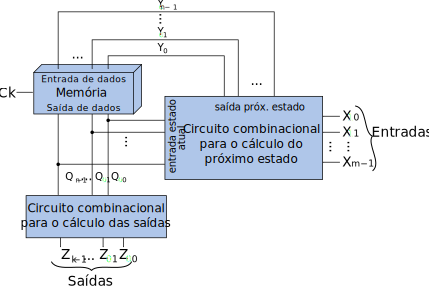
\includegraphics[scale=1.3]{images/state_machine_general}
\end{center}

Na aula passada, vimos casos específicos de máquinas de estado chamadas
\emph{contadores}, onde o único sinal de entrada é o \emph{clock}, e cada
transição é feita em uma borda do clock (seja de subida ou de descida, a
dependender dos flip-flops empregados).

Hoje veremos os casos em que outras entradas, além do clock, influenciam
na transição entre estados.

\section{Projeto de máquinas de estado}

\begin{ex}
Faça um contador progressivo/regressivo para um código de Gray de $2$ bits.

A sequência de Gray para $2$ bits é: $00$, $01$, $11$, $10$.

O contador terá $2$ entradas:
\begin{itemize}
\item $Ck$ -- clock
\item $X$ -- indica se a transição será feita para o numeral \emph{seguinte},
             se $X = 1$, ou para o \emph{anterior}, se $X = 0$, na sequência
             de Gray.
\end{itemize}
\end{ex}

\passo{1} diagrama de estados.
\begin{center}
\begin{tikzpicture}[shorten >=1pt,node distance=3cm,on grid,auto]
\tikzset{>=stealth}
  \node[state] (00) {$00$};
  \node[state] (01) [below right=of 00] {$01$};
  \node[state] (10) [below left=of 00] {$10$};
  \node[state] (11) [below right=of 10] {$11$};
  \path[->] (00) edge [pos=.85,bend left=15,sloped] node {$X=0$} (10);
  \path[->] (00) edge [bend left=15] node {$X=1$} (01);
  \path[->] (01) edge [pos=.15,bend left=15,sloped] node {$X=0$} (00);
  \path[->] (01) edge [bend left=15] node {$X=1$} (11);
  \path[->] (11) edge [pos=.85,bend left=15,sloped] node {$X=0$} (01);
  \path[->] (11) edge [bend left=15] node {$X=1$} (10);
  \path[->] (10) edge [pos=.15,bend left=15,sloped] node {$X=0$} (11);
  \path[->] (10) edge [bend left=15] node {$X=1$} (00);
\end{tikzpicture}
\end{center}

\passo{2} tabelas verdade para os bits do próximo estado
(tabelas de transição).
Estado atual: $Q_1$, $Q_0$. Próximo estado: $Y_1$, $Y_0$.
\begin{center}
\begin{tabular}{ccc||cc}
 $Q_1$ & $Q_0$ & $X$ & $Y_1$ & $Y_0$ \\
\hline
 0 & 0 & 1 & 0 & 1 \\
 0 & 0 & 0 & 1 & 0 \\
 0 & 1 & 1 & 1 & 1 \\
 0 & 1 & 0 & 0 & 0 \\
 1 & 1 & 1 & 1 & 0 \\
 1 & 1 & 0 & 0 & 1 \\
 1 & 0 & 1 & 0 & 0 \\
 1 & 0 & 0 & 1 & 1 
\end{tabular}
\end{center}

\passo{3} obter expressões para $Y_1$ e $Y_0$.

\hfill%
\begin{minipage}{0.4\textwidth}
\begin{center}
Mapa de Karnaugh para $Y_1$

\begin{Karnaughvuit}{$X$}{\raisebox{0.5\baselineskip}{$Q_1 Q_0$}}
    \contingut{1,0,1,0,0,1,0,1}
    \implicantcostats{0}{2}{red}
    \implicant{5}{7}{green}
\end{Karnaughvuit}

$Y_1 = \Not{X}\Not{Q_0} + X Q_0 = \Not{X \Xor Q_0}$
\end{center}
\end{minipage}%
\hfill%
\begin{minipage}{0.4\textwidth}
\begin{center}
Mapa de Karnaugh para $Y_0$

\begin{Karnaughvuit}{$X$}{\raisebox{0.5\baselineskip}{$Q_1 Q_0$}}
    \contingut{0,0,1,1,1,1,0,0}
    \implicant{3}{2}{red}
    \implicant{4}{5}{green}
\end{Karnaughvuit}

$Y_1 = X\Not{Q_1} + \Not{X} Q_1 = X \Xor Q_1$
\end{center}
\end{minipage}
\hspace*{\fill}

\passo{4} diagrama do circuito.

\begin{tikzpicture}[x=2\baselineskip,y=2\baselineskip]
\tikzstyle{branch}=[fill,shape=circle,minimum size=4pt,inner sep=0pt]
\Dff{2}{5}{dff1}
\Dff{6}{5}{dff2}
\node (Ck) at (0,3) {$Ck$};
\node (X) at (13,2) {$X$};
\node[xor gate US,draw,logic gate inputs=nn,thick,right=of dff2q,
      xshift=2\baselineskip,yshift=-\baselineskip,thick,right=of dff2q,
      rotate=90,scale=1.3]
     (xor) {};
\node[xnor gate US,draw,logic gate inputs=nn,thick,
      anchor=input 1,rotate=90,scale=1.3] at ($(xor.input 1)+(1.5,0)$)
     (xnor) {};
\draw (Ck) -| node[branch] {} ($(dff1ck)-(0.5,0)$) -- ++(0.5,0);
\draw (Ck) -| ($(dff2ck)-(0.5,0)$) -- ++(0.5,0);
\tikzset{>={triangle 45}}
\draw[->] (dff1q.east) -- ++(0.5,0) --
      node[branch,pos=1] (branch1) {} ++(0,-2.5) --
      node[below,pos=1] (Q1) {$Q_1$} ++(0,-2);
\draw[->] (dff2q.east) -- ++(0.5,0) --
      node[branch,pos=1] (branch2) {} ++(0,-3.5) --
      node[below,pos=1] (Q0) {$Q_0$} ++(0,-1);
\draw (branch1) -| (xor.input 1);
\draw[->] (X) -- ($(X)+(-1,0)$); \draw ($(X)+(-1,0)$) -| (xor.input 2);
\draw (xor.output) |- ($(dff2d.west)+(-0.5,1)$) |- (dff2d.west);
\draw (branch2) -| (xnor.input 2);
\draw (X) -| node[branch] {} (xnor.input 1);
\draw (xnor.output) |- ($(dff1d.west)+(-0.5,1.5)$) |- (dff1d.west);
\end{tikzpicture}

\begin{ex}
Projete uma máquina de venda de água e refrigerante que aceite moedas de
R\$ 0,50 e R\$ 1,00 e permita que o comprador escolha \emph{água} se as
moedas inseridas totalizam R\$1,50 ou mais ou \emph{refrigerante} se o
total depositado é de R\$2,00 ou mais.

A detecção de moedas é feira por um dispositivo eletromecânico que possui
duas saídas:
\begin{itemize}
  \item $Ck$ -- que identifica por meio de uma transição $1 \rightarrow 0$
        (borda de descida) quando uma moeda inserida é considerada válida.
  \item $X$ -- que é $0$ se a moeda inserida é de 50 centavos ou $1$ se
        a moeda é de um real.
\end{itemize}

Para simplificar, considere que a máquina não dá troco nem mostra o valor
total inserido.
\end{ex}

\passo{1} diagrama de estados.

Primeiramente, vamos fazer o diagrama colocando em cada estado o valor total
(em R\$) de moedas introduzidas e em cada transição (setas) o valor da moeda
a ser inserida para que tenhamos a transição. Começamos com um total de
R\$ 0,00.

\begin{center}
\begin{tikzpicture}[shorten >=1pt,node distance=7\baselineskip and 10\baselineskip,on grid,auto,very thick]
\tikzset{>=stealth}
\begin{scope}[every node/.style={draw,minimum size=3cm,inner sep=0.9em}]
%\begin{scope}[every node/.style={draw,fill=gray!40,circle,inner sep=0.75em}]
  \node[state] (000) {R\$ 0,00};
  \node[state] (050) [right=of 000] {R\$ 0,50};
  \node[state] (100) [right=of 050] {R\$ 1,00};
\end{scope}
  \node[state with output,inner sep=0.5em] (150) [below=of 050]
       {R\$ 1,50 \nodepart{lower} só água};
  \node[state with output] (200) [below=of 100]
       {$\ge$ R\$ 2,00 \nodepart{lower} {\smallágua, refri}};
  \path[->] (000) edge node {+R\$ 0,50} (050);
  \path[->] (000) edge [bend left=30] node {+R\$ 1,00} (100);
  \path[->] (050) edge node {+R\$ 0,50} (100);
  \path[->] (050) edge [left] node {+R\$ 1,00} (150);
  \path[->] (100) edge [sloped,pos=.75] node {+R\$ 0,50} (150);
  \path[->] (100) edge node {+R\$ 1,00} (200);
  \path[->] (150) edge node {+R\$ 0,50} (200);
  \path[->] (150) edge [below,bend right=15] node {+R\$ 1,00} (200);
  \path[->] (200) edge [in=15,out=45,loop] node {+R\$ 0,50} (200);
  \path[->] (200) edge [in=-30,out=0,loop] node {+R\$ 1,00} (200);
\end{tikzpicture}
\end{center}

Agora, vamos transformar cada estado em um número binário, assim como
as transições, e vamos determinar também os valores das saídas $A$ (água)
e $R$ (refrigerante) para cada estado. Escolheremos o estado inicial como
sendo a um código binário que corresponda a \emph{zero}. Como temos $5$
estado, precisaremos de $3$ bits para identificar cada um dos estados.

\begin{center}
\begin{tikzpicture}[shorten >=1pt,node distance=7\baselineskip and 10\baselineskip,on grid,auto,very thick]
\tikzset{>=stealth}
\begin{scope}[every node/.style={inner sep=0.4ex}]
  \node[state with output,align=center] (000)
       {\raisebox{0.75ex}{\Large{000}} \nodepart{lower} $A=0$ \\ $R=0$};
  \node[state with output,align=center] (050) [right=of 000]
       {\raisebox{0.75ex}{\Large{001}} \nodepart{lower} $A=0$ \\ $R=0$};
  \node[state with output,align=center] (100) [right=of 050]
       {\raisebox{0.75ex}{\Large{010}} \nodepart{lower} $A=0$ \\ $R=0$};
  \node[state with output,align=center] (150) [below=of 050]
       {\raisebox{0.75ex}{\Large{011}} \nodepart{lower} $A=1$ \\ $R=0$};
  \node[state with output,align=center] (200) [below=of 100]
       {\raisebox{0.75ex}{\Large{100}} \nodepart{lower} $A=1$ \\ $R=1$};
\end{scope}
  \path[->] (000) edge node {$X = 0$} (050);
  \path[->] (000) edge [bend left=30] node {$X = 1$} (100);
  \path[->] (050) edge node {$X = 0$} (100);
  \path[->] (050) edge [left] node {$X = 1$} (150);
  \path[->] (100) edge [sloped,pos=.75] node {$X = 0$} (150);
  \path[->] (100) edge node {$X = 1$} (200);
  \path[->] (150) edge node {$X = 0$} (200);
  \path[->] (150) edge [below,bend right=15] node {$X = 1$} (200);
  \path[->] (200) edge [in=15,out=45,loop] node {$X = 0$} (200);
  \path[->] (200) edge [in=-30,out=0,loop] node {$X = 1$} (200);
\end{tikzpicture}
\end{center}

\passo{2} Tabelas de transição.

\begin{center}
\begin{tabular}{c|c c c||c c c}
     & \multicolumn{3}{c||}{estado atual} & \multicolumn{3}{c}{próx. estado} \\
 $X$ & $Q_2$ & $Q_1$ & $Q_0$ & $Y_2$ & $Y_1$ & $Y_0$ \\
\hline
 0 & 0 & 0 & 0 & 0 & 0 & 1 \\
 0 & 0 & 0 & 1 & 0 & 1 & 0 \\
 0 & 0 & 1 & 0 & 0 & 1 & 1 \\
 0 & 0 & 1 & 1 & 1 & 0 & 0 \\
 0 & 1 & 0 & 0 & 1 & 0 & 0 \\
 1 & 0 & 0 & 0 & 0 & 1 & 0 \\
 1 & 0 & 0 & 1 & 0 & 1 & 1 \\
 1 & 0 & 1 & 0 & 1 & 0 & 0 \\
 1 & 0 & 1 & 1 & 1 & 0 & 0 \\
 1 & 1 & 0 & 0 & 1 & 0 & 0 \\
\end{tabular}
\end{center}

\passo{3} obtenção de expressões para $Y_2$, $Y_1$ e $Y_0$.

\noindent
\begin{minipage}{0.275\textwidth}
\begin{Karnaugh}{$X Q_2$}{\raisebox{0.5\baselineskip}{$Q_1 Q_0$}}
  \contingut{0,0,0,1,1,\dontcare,\dontcare,\dontcare,0,0,1,1,1,\dontcare,\dontcare,\dontcare}
  \implicant{15}{10}{red}
  \implicant[3pt]{4}{14}{green}
  \implicant{3}{7}{blue}
\end{Karnaugh}

\vspace{-1.3\baselineskip}

$Y_2 = Q_1 Q_0 + Q_2 + X Q_1$

\end{minipage}%
\hfill
\begin{minipage}{0.33\textwidth}
\begin{Karnaugh}{$X Q_2$}{\raisebox{0.5\baselineskip}{$Q_1 Q_0$}}
  \contingut{0,1,1,0,0,\dontcare,\dontcare,\dontcare,1,1,0,0,0,\dontcare,\dontcare,\dontcare}
  \implicant{8}{9}{red}
  \implicant[2pt]{1}{9}{green}
  \implicant{2}{6}{blue}
\end{Karnaugh}

\vspace{-1.3\baselineskip}

$Y_1 = \Not{Q_1} Q_0 + \Not{X} Q_1 \Not{Q_0} + X \Not{Q_2} \; \Not{Q_1}$

\end{minipage}%
\hfill
\begin{minipage}{0.33\textwidth}
\begin{Karnaugh}{$X Q_2$}{\raisebox{0.5\baselineskip}{$Q_1 Q_0$}}
  \contingut{1,0,1,0,0,\dontcare,\dontcare,\dontcare,0,1,0,0,0,\dontcare,\dontcare,\dontcare}
  \implicantcostats{0}{2}{red}
  \implicant{13}{9}{blue}
\end{Karnaugh}

\vspace{-1.3\baselineskip}

$Y_0 = X \Not{Q_1} Q_0 + \Not{X} \; \Not{Q_2} \; \Not{Q_0}$

\end{minipage}%

\passo{4} diagrama do circuito.

Usaremos tanto as saídas $Q$ quanto as saídas $\Not{Q}$ de cada flip-flop.

Por enquanto, faremos o circuito sem a detecção dos estados finais (só água
e água/re\-fri\-ge\-ran\-te). Adicionaremos a detecção destes estados nas
próximas etapas.

\newenvironment{vendingmachine}{
\noindent
\begin{tikzpicture}[x=1.5\baselineskip,y=1.5\baselineskip]
\tikzstyle{branch}=[fill,shape=circle,minimum size=4pt,inner sep=0pt]

\Dff{2}{5}{dff2}
\Dff{5.5}{5}{dff1}
\Dff{9}{5}{dff0}

\tikzset{>={triangle 45}}

\node (Ck) at (0,3) {$Ck$};
\node (X) at (0,1.5) {$X$}; \draw[->] (X) -- ++(1.5,0);
\node[not gate US,draw] (not) at (10,2) {};
\draw (not.input) -| ++(-0.5,-0.5) -- node[branch,pos=0] (branchX) {} (X);
\coordinate (nX) at (not.output);

\draw (Ck) -| ($(dff0ck.west)+(-0.25,0)$) -- (dff0ck.west);
\draw (Ck) -| node[branch] {} ($(dff1ck.west)+(-0.25,0)$) -- (dff1ck.west);
\draw (Ck) -| node[branch] {} ($(dff2ck.west)+(-0.25,0)$) -- (dff2ck.west);

}
{
\node[branch] (pQ2) at ($(Q2)+(0,1.5)$) {};
\node[branch] (pQ1) at ($(Q1)+(0,2.5)$) {};
\node[branch] (pQ0) at ($(Q0)+(0,3.5)$) {};

\draw (dff2nq.east) -- ++(-0.1,0) -|
      coordinate[pos=1] (nQ2) ($(pQ2)+(-0.4,-0.4)$);
\draw (dff1nq.east) -- ++(-0.1,0) -|
      coordinate[pos=1] (nQ1) ($(pQ1)+(-0.4,-0.4)$);
\draw (dff0nq.east) -- ++(-0.1,0) -|
      coordinate[pos=1] (nQ0) ($(pQ0)+(-0.4,-0.4)$);

\node[and gate US,thick,draw,logic gate inputs=nnn,right=of dff0q,
      yshift=-0.5\baselineskip,
      rotate=90]%,scale=1.3]
     (and01) {};

\node[and gate US,thick,draw,logic gate inputs=nnn,right=of and01,
      anchor=output,rotate=90]%,scale=1.3]
     (and02) {};

\node[or gate US,thick,draw,logic gate inputs=nn,rotate=90,yscale=1.5,scale=1.75,
      anchor=base west]
     (or0) at ($(and01.output)!0.5!(and02.output)+(0,1)$) {};

\draw (X) -| node[branch] {} (and01.input 1);
\draw (pQ0) -| node[branch] {} (and01.input 2);
\draw (nQ1) -| node[branch] {} (and01.input 3);

\draw (nX) -| node[branch] {} (and02.input 1);
\draw (nQ0) -| node[branch] {} (and02.input 2);
\draw (nQ2) -| node[branch] {} (and02.input 3);

\draw (and01.output) -- ++(0,0.5) -| (or0.input 1);
\draw (and02.output) -- ++(0,0.5) -| (or0.input 2);
\draw (or0.output) -- ++(0,0.5) -- node[below] {$Y_0$} ++(-4.35,0)
      |- (dff0d.west) -- ++(0.1,0);

\node[and gate US,thick,draw,logic gate inputs=nn,right=of and02,
      anchor=output,rotate=90,scale=1.35]
     (and11) {};

\node[and gate US,thick,draw,logic gate inputs=nnn,right=of and11.south west,
      xshift=1em,
      anchor=south west,rotate=90]%,scale=1.3]
     (and13) {};

\node[and gate US,thick,draw,logic gate inputs=nnn,
      anchor=output,rotate=90]%,scale=1.3]
     (and12) at ($(and11.south west)!0.5!(and13.north west)+(0,-0.25)$) {};

\node[or gate US,thick,draw,logic gate inputs=nnn,rotate=90,yscale=1.4,scale=1.35,
      anchor=base west]
     (or1) at ($(and11.output)!0.5!(and13.output)+(0,1)$) {};

\draw (pQ0) -| node[branch] {} (and11.input 1);
\draw (nQ1) -| node[branch] {} (and11.input 2);

\draw (nX) -| node[branch] {} (and12.input 1);
\draw (nQ0) -| (and12.input 2);
\draw (pQ1) -| node[branch] {} (and12.input 3);

\draw (X) -| (and13.input 1);
\draw (nQ1) -| node[branch] {} (and13.input 2);
\draw (nQ2) -| (and13.input 3);

\draw (and11.output) -- ++(0,0.5) -| (or1.input 1);
\draw (and12.output) -- (or1.input 2);
\draw (and13.output) -- ++(0,0.5) -| (or1.input 3);
\draw (or1.output) -- ++(0,1.0) -- node[below,pos=0.15] {$Y_1$} ++(-10.75,0)
      |- (dff1d.west) -- ++(0.1,0);

\node[and gate US,thick,draw,logic gate inputs=nn,right=of and13,
      anchor=output,rotate=90,scale=1.35]
     (and21) {};

\node[and gate US,thick,draw,logic gate inputs=nn,right=of and21,
      xshift=1em,
      anchor=output,rotate=90,scale=1.35]
     (and22) {};

\node[or gate US,thick,draw,logic gate inputs=nnn,rotate=90,yscale=1.5,
      scale=1.3,anchor=base west]
     (or2) at ($(and21.output)!0.5!(and22.output)+(0,1)$) {};

\draw (pQ0) -| (and21.input 1);
\draw (nQ1) -| (and21.input 2);

\draw (pQ2) -| (or2.input 2);

\draw (nX) -| (and22.input 1);
\draw (pQ1) -| (and22.input 2);

\draw (and21.output) -- ++(0,0.5) -| (or2.input 1);
\draw (and22.output) -- ++(0,0.5) -| (or2.input 3);
\draw (or2.output) -- ++(0,1.5) -- node[below,pos=0.1] {$Y_2$} ++(-17.5,0)
      |- (dff2d.west) -- ++(0.1,0);
\end{tikzpicture}
}

\begin{vendingmachine}

\draw[->] (dff2q.east) -- ++(-0.1,0) -- ++(0.6,0) --
          node[pos=1,below] (Q2) {$Q_2$} ++(0,-7.5);
\draw[->] (dff1q.east) -- ++(-0.1,0) -- ++(0.6,0) --
          node[pos=1,below] (Q1) {$Q_1$} ++(0,-7.5);
\draw[->] (dff0q.east) -- ++(-0.1,0) -- ++(0.6,0) --
          node[pos=1,below] (Q0) {$Q_0$} ++(0,-7.5);

\end{vendingmachine}

Precisamos, agora, de um circuito combinacional para permitir a seleção de
\emph{água} quando o estado for 011 ou 100 e \emph{refrigerante} quando o
estado for 100. Teremos os seguintes mapas de Karnaugh para as funções lógicas
$A$ e $R$, que dependem dos bits de estado $Q_2$, $Q_1$ e $Q_0$:

%\hfill
\begin{minipage}{0.4\textwidth}
\begin{center}
\begin{Karnaughvuit}{$Q_2$}{\raisebox{0.5\baselineskip}{$Q_1 Q_0$}}
    \contingut{0,0,0,1,1,\dontcare,\dontcare,\dontcare}
    \implicant{3}{7}{red}
    \implicant{4}{6}{green}
\end{Karnaughvuit}

\vspace{-1.3\baselineskip}

$A = Q_2 + Q_1 Q_0$
\end{center}
\end{minipage}%
\hfill%
\begin{minipage}{0.4\textwidth}
\begin{center}
\begin{Karnaughvuit}{$Q_2$}{\raisebox{0.5\baselineskip}{$Q_1 Q_0$}}
    \contingut{0,0,0,0,1,\dontcare,\dontcare,\dontcare}
    \implicant{4}{6}{green}
\end{Karnaughvuit}

\vspace{-1.3\baselineskip}

$R = Q_2$
\end{center}
\end{minipage}%
\hspace*{\fill}\\

O circuito completo da máquina de estados é:\\

\begin{vendingmachine}

\draw[-] (dff2q.east) -- ++(-0.1,0) -- ++(0.6,0) --
          node[pos=1] (Q2) {\hspace{2em}$Q_2$} ++(0,-7.5);
\draw[-] (dff1q.east) -- ++(-0.1,0) -- ++(0.6,0) --
          node[pos=1] (Q1) {\hspace{2em}$Q_1$} ++(0,-7.5);
\draw[-] (dff0q.east) -- ++(-0.1,0) -- ++(0.6,0) --
          node[pos=1] (Q0) {\hspace{2em}$Q_0$} ++(0,-7.5);

\draw[->] (Q2.north) -- node[branch,pos=1] (branchR) {} ++(0,-2) --
          node[pos=1,below] (R) {$R$} ++(0,-4.5);
\node[and gate US,draw,thick,logic gate inputs=nnn,anchor=output,rotate=-90]
     (andA) at ($(Q1.north)!0.5!(Q0.north)+(0,-3)$) {};
\draw (Q1.north) |- ($(andA.input 3)+(0,0.5)$) -- ++(0,-0.5);
\draw (Q0.north) |- ($(andA.input 1)+(0,0.5)$) -- ++(0,-0.5);
\node[or gate US,draw,thick,logic gate inputs=nnnn,anchor=input 1,rotate=-90]
     (orA) at ($(andA.output)+(0,-0.5)$) {};
\draw (andA.output) -- (orA.input 1);
\draw (branchR) -| (orA.input 4);
\node[anchor=north] (A) at ($(orA.output |- R.north)$) {$A$};
\draw[->] (orA.output) -- (A);
\end{vendingmachine}

\end{document}
